% Activate the following line by filling in the right side. If for example the name of the root file is Main.tex, write
% "...root = Main.tex" if the chapter file is in the same directory, and "...root = ../Main.tex" if the chapter is in a subdirectory.
 
%!TEX root =  testMain.tex

\chapter[Robberies in ``real'' locations]{Robberies}

In the previous chapters, we moved from a non-spatial simulation, to a very simple spatial simulation. In the simple spatial simulations, agents move through an environment, but that environment is very trivial - there are two houses, that is about it. A simulation with non-trivial environment might lead to more uncertainty, and require more interesting agent-behaviours that might prove challenging for the Bayesian Network. Additionally, by implementing non-trivial environments, we move closer to the state-of-the-art agent models for modelling crime cases.


Research questions for this chapter:

\begin{itemize}
\item Can we create a simulation that somewhat reflects a real world location?
\item Can we create an automatic BN from this simulation that fulfils the criteria we set out for it?
\end{itemize}



\section{Introduction}
We take the theme of the robbery from last chapter, and make it a street robbery. Two agents are walking around at the Grote Markt (the central town square in Groningen). One of the agents is old

\section{Methods}

We wrote a method to convert screenshots of maps into an agent-readable environment. The maps were screenshotted from \url{http://maps.stamen.com/terrain/#18/53.21618/6.57225} and converted into greyscale. Then, they were transformed into a grid of a given size. The average greyscale value of each cell in the grid was taken and coded as either `accessible' or `non-accessible'. On the greyscale map, the color of the buildings was in the range of (189, 199) - cells within this range were coded as `inaccessible', since agents cannot walk through buildings. All other cells were `accessible'. This resulted in a map shared by all agents that constrained their movements. There are 8 cameras placed randomly on the `accessible' cells on the map, each with a visual radius of 15. Additionally, we used this map to calculate the sight lines of both cameras and agents. An agent or a camera cannot see another agent if there is an `inaccessible' grid cell on the sight line between the two.

The agents have some other features than before. Every agent has an age, to determine whether they are vulnerable or not - old people are considered more vulnerable. Every agent also has an object of a certain value, the thief's object has a value of -1, and the other agent's object has a value of 1000, to make it a tempting target. An agent decides if it wants to steal something by making a very simple risk-calculation based on their risk threshold: if the object is more expensive than their risk threshold, they will attempt to steal it (contributing to `motive'). Every agent also has a goal state, this is the location at the edge of the map. When they enter their goal state, they are essentially removed from the simulation, as they leave the relevant area. Every simulation was run for 100 timesteps, or until both agents are in their goal states. The simulation itself was ran 2500 iterations. The behaviour of the agents is shown in Figure~\ref{behaviourGM}. Agents are placed randomly on the map initially.


\begin{figure}[htbp]
\begin{center}
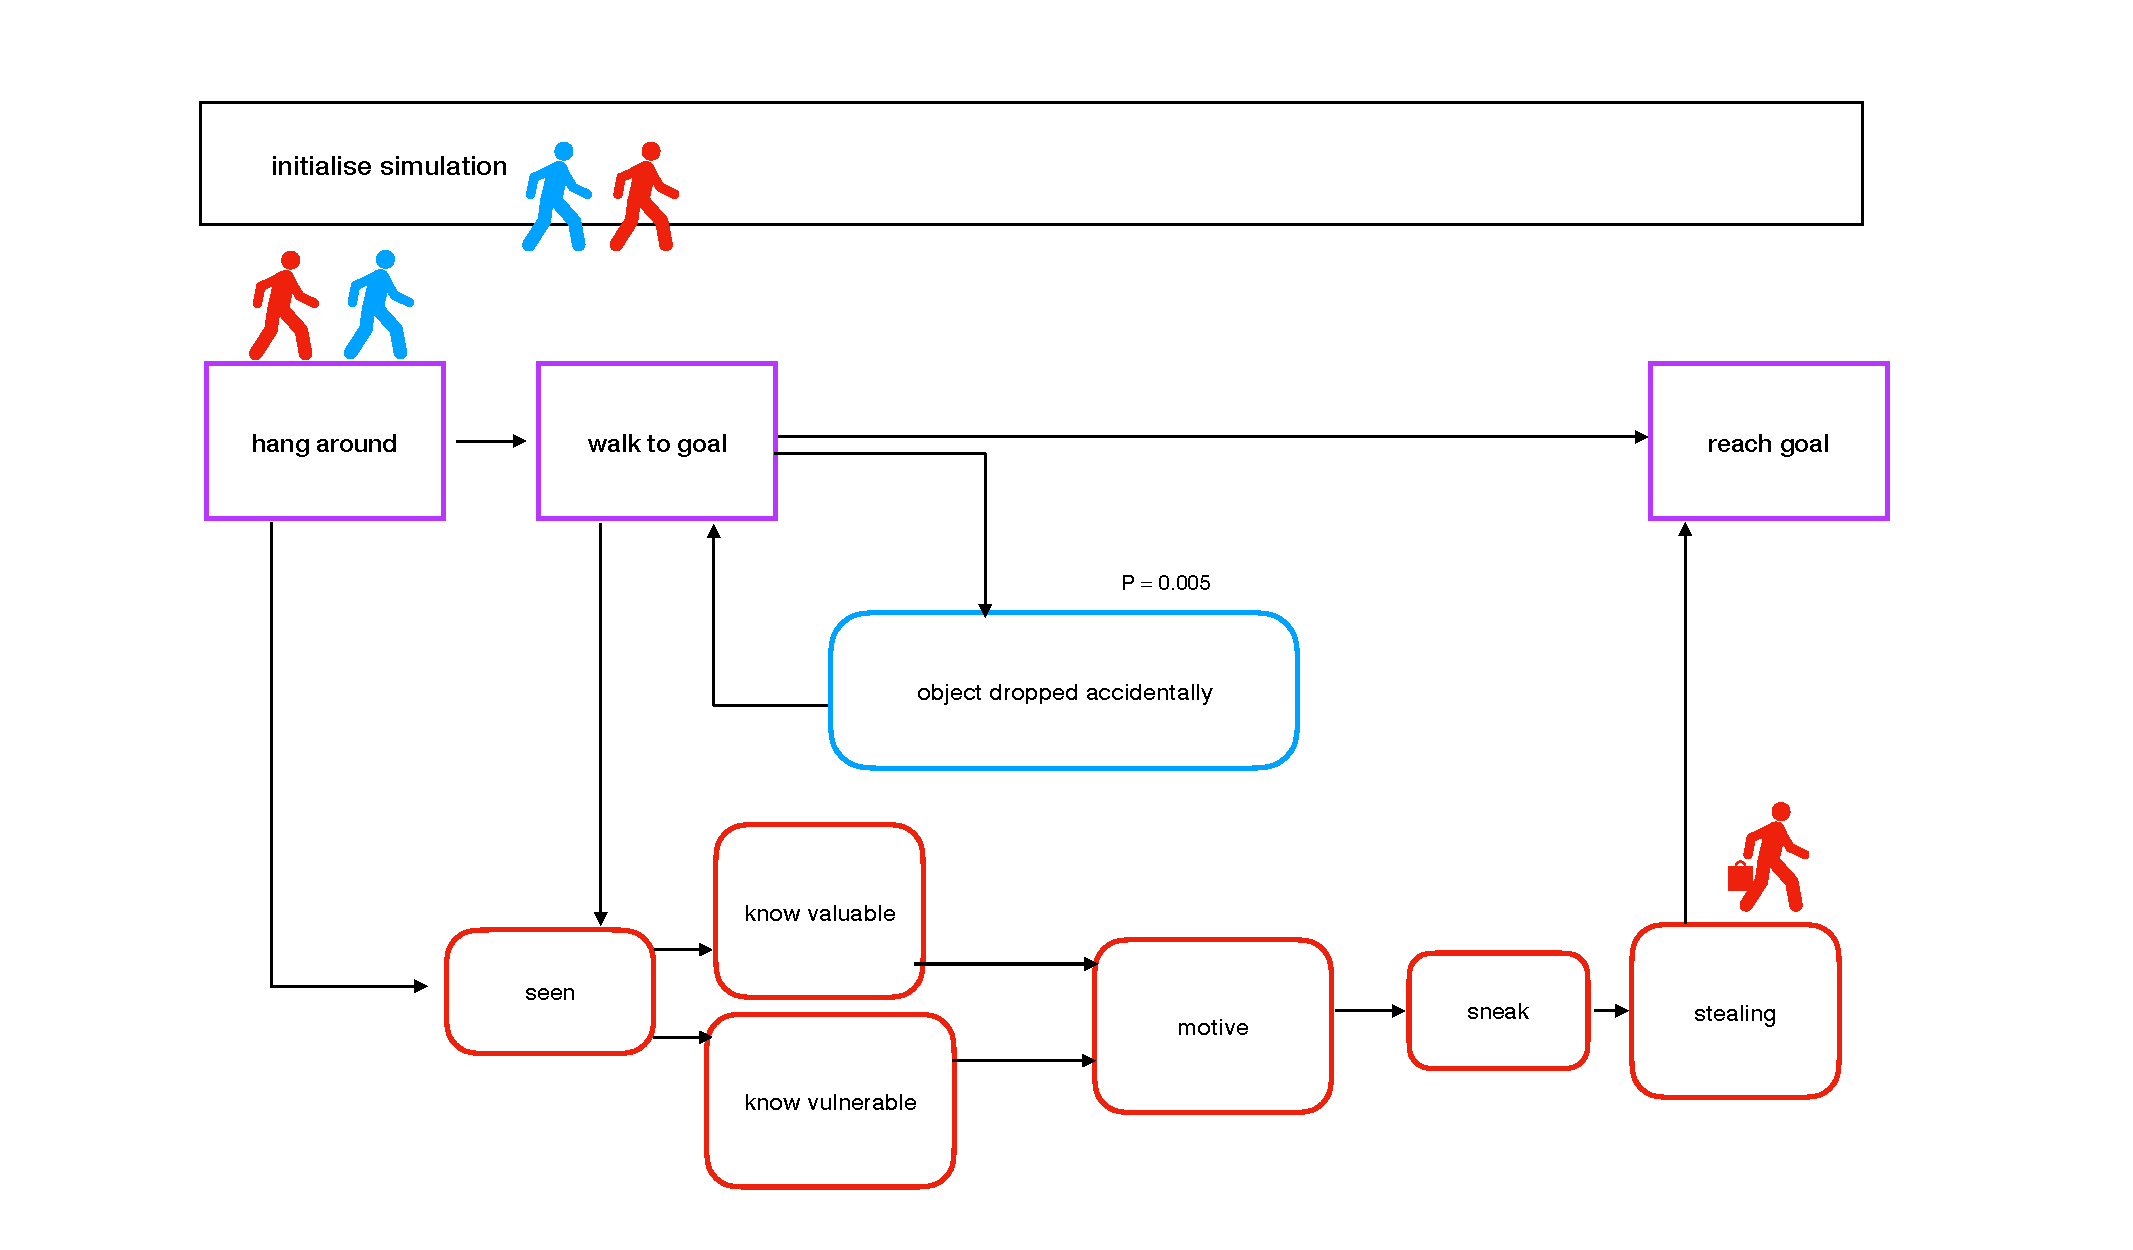
\includegraphics[width=\linewidth]{images/grotemarkt.pdf}
\end{center}
\caption{The behaviour of the agents. The nodes with rounded edges correspond to the nodes in the Bayesian Network.}
\label{behaviourGM}
\end{figure}

\begin{adjustbox}{center}
\footnotesize
%\centering
\begin{tabular}{|l|l|}
 \hline
 RV &Operationalization\\
 \hline
\hline
\end{tabular}
\end{adjustbox}



\begin{figure}[htbp]
\begin{center}
\begin{subfigure}{.5\textwidth}
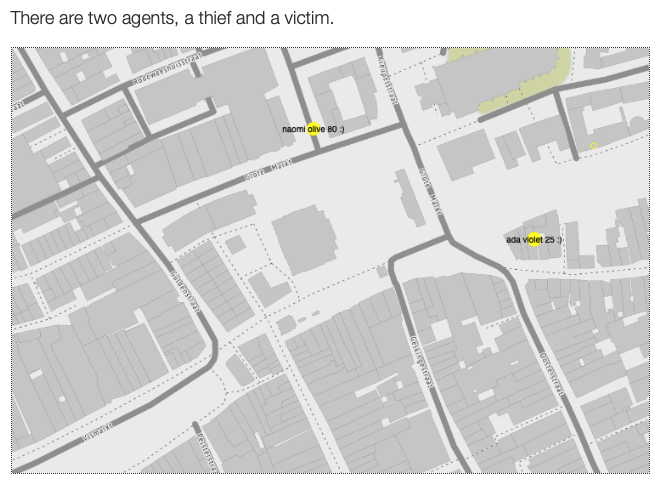
\includegraphics[width=\linewidth]{images/grotemarktmap.png}
\caption{map of environment - 2 agents}
\end{subfigure}%
\begin{subfigure}{.5\textwidth}
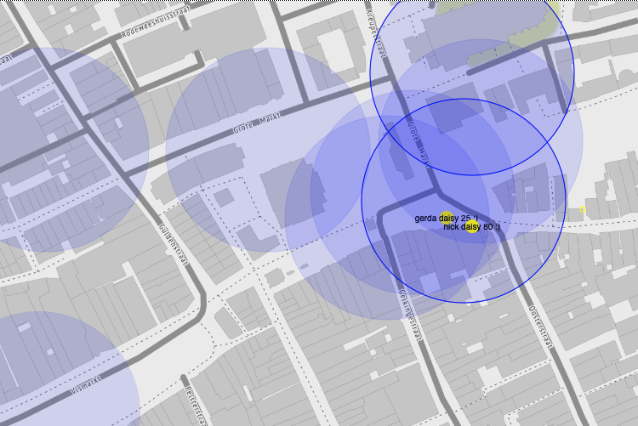
\includegraphics[width=\linewidth]{images/grotemarktCameras.png}
\caption{Camera locations are randomly initialized}
\end{subfigure}%
\label{groteMarkt}
\caption{The Grote Markt environment}
\end{center}
\end{figure}



\section{Results}

The network is shown in Figure~\ref{groteMarkperfo}.
\begin{figure}[htbp]
\begin{center}
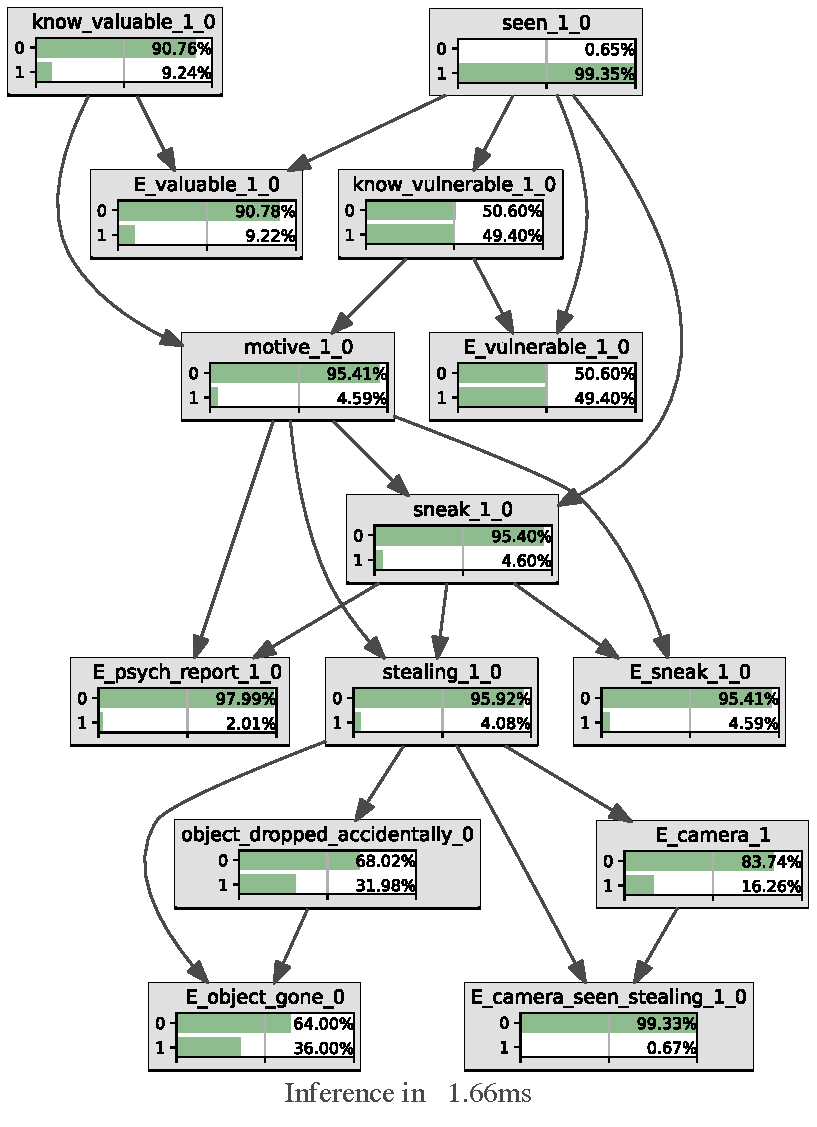
\includegraphics[width=.7\linewidth]{../experiments/GroteMarkt/bnImage/BNIMAGEGroteMarkt.pdf}
\caption{Bayesian Network}
\label{groteMarktperfo}
\end{center}
\end{figure}

\subsection{Structural Criteria}
\begin{enumerate}
\item Hypotheses are ordered temporally. Following the cause-consequence idiom.
\item Evidence connects to hypotheses.
\item Relevance: All relevant events are in the BN, all irrelevant events are outside of the BN.
\item Independent events are not connected to each other.
\end{enumerate}

\subsection{Performance Criteria}
\begin{enumerate}
\item Accuracy and RMSE.

The accuracy of the network is 92.3\%, which is better than in the previous networks. The RMSE is 0.078. 
\item Correspondence.

The frequency of events in the network (without evidence set) correspond to the frequency of events in the simulation within ±0.001.

\begin{table}
\centering
\begin{tabular}{|c|c|c|}
 \hline
 Conclusion & Frequency P(event) & BN P(event)\\
 \hline
seen   & 0.5415& 0.5415\\
know valuable & 0.2285 &  0.2286\\
know vulnerable & 0.5415 &  0.5414\\
motive & 0.2285 &  0.2285\\
sneak & 0.2285 & 0.2284\\
stealing & 0.19 & 0.1900\\
accident & 0.1515 & 0.1517 \\
E psych report & 0.1815 &  0.1814\\
E camera & 0.999 & 0.9987\\ 
E object gone & 0.3415 & 0.3414 \\
 \hline
\label{test}
\end{tabular}
\caption{Do we match with the frequencies?}
\end{table}


\item Sensitivity Values of Output Node.
\item Evidence updates the posterior in the correct direction.
We tell the following story with the evidence
\begin{figure}[htbp]
 \centering
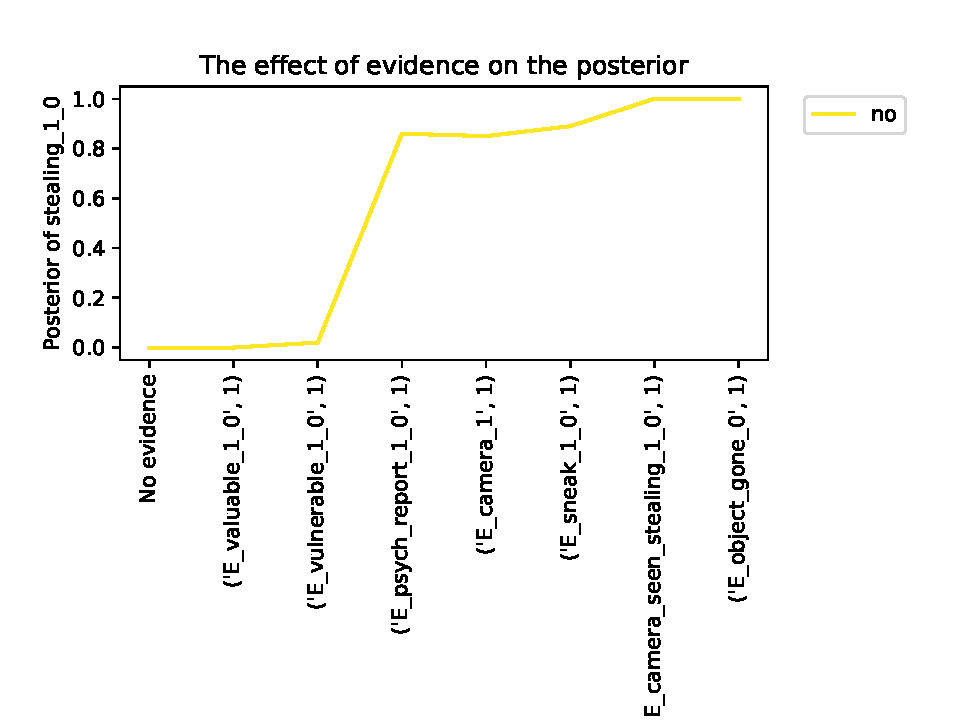
\includegraphics[width=0.6\linewidth]{../experiments/GroteMarkt/plots/posterior_base_networkGroteMarkt.pdf}
\caption{ Progression of evidence resulting in changing the posterior}
\label{baseposterior}
\end{figure}%
\end{enumerate}

\subsection{Human Criteria}
\begin{enumerate}
\item How robust is the network against a loss of precision?

\begin{figure}[htbp]
\begin{center}
\begin{subfigure}{.5\textwidth}
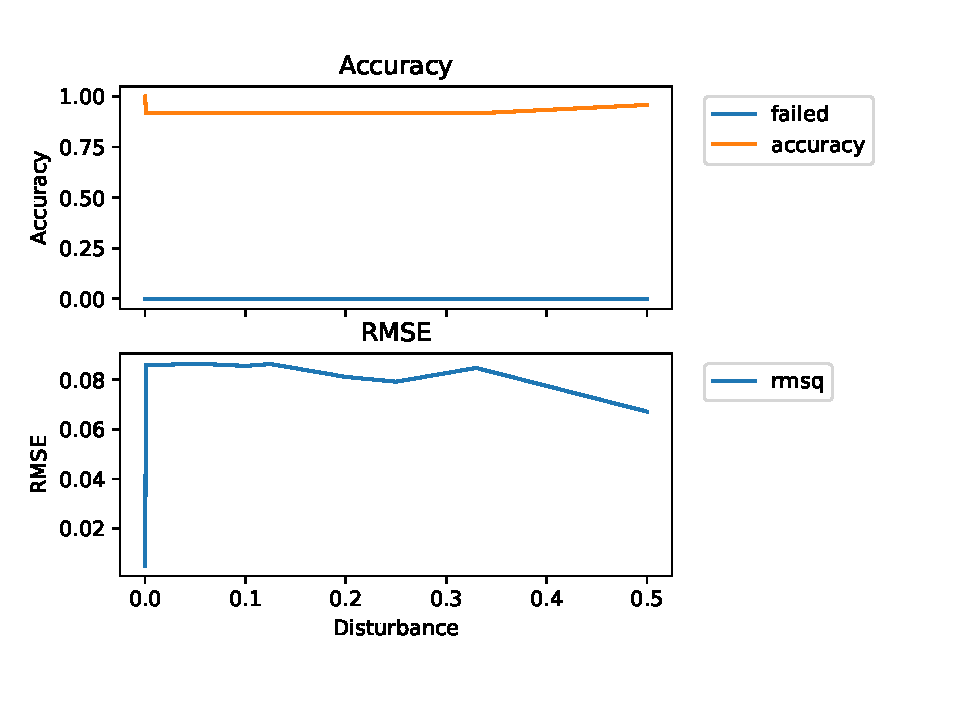
\includegraphics[width=0.9\linewidth]{../experiments/GroteMarkt/plots/performance_GroteMarkt.pdf}
\caption{Network Under Disturbance.}
\label{dist}
\end{subfigure}%
\begin{subfigure}{.5\textwidth}
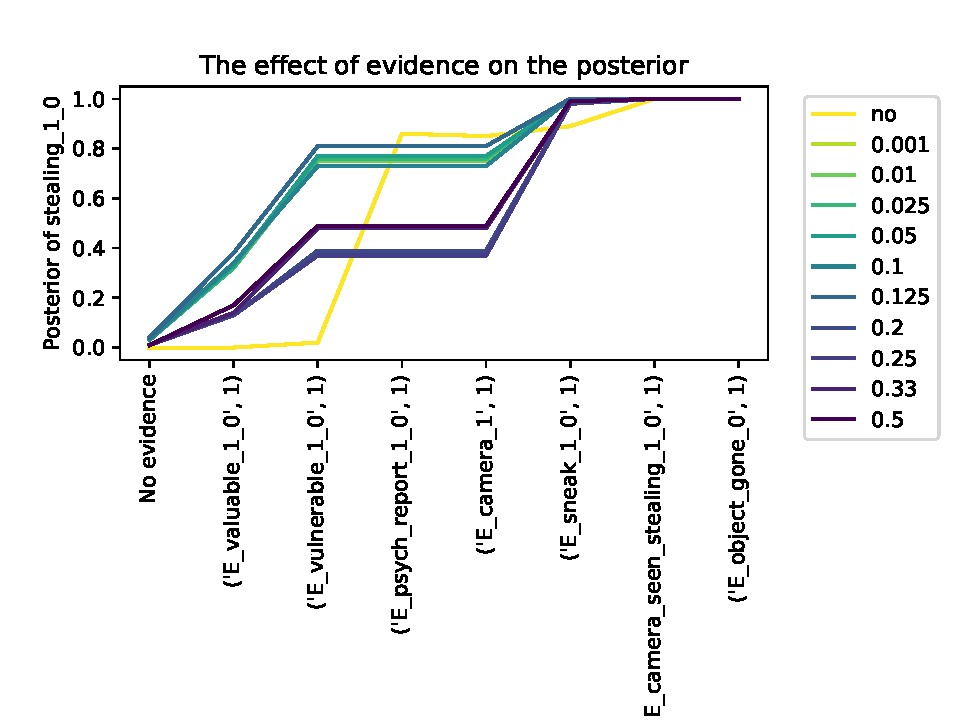
\includegraphics[width=0.9\linewidth]{../experiments/GroteMarkt/plots/posterior_GroteMarkt.pdf}
\caption{ Progression of evidence resulting in changing the posterior}
\label{post}
\end{subfigure}
\end{center}
\caption{Loss of precision in networks.}
\end{figure}

\item Could a human find these probabilities?
\item Can a human determine the correct independence relations?
\end{enumerate}




\section{Discussion}
We have shown in this chapter that the specific geometry of simulation matters a lot for the results of the simulation. 

If we haven't implemented camera evidence yet, but only a psych report and the victim knowing that it lost the object, then the posterior of stealing goes to 1, but the accuracy of the network is 0.6. bas, because it cnnot distinguish cases of stealing from cases of dropping based on the evidence that we have.
This network has the risk of convicting someone based on a mistake!!! The victim can drop the object, but if the 

\subsection{Limitations of the simulation.}
This simulation should be seen as a preliminary for further research, as it is lacking in several aspects: the environment is still too simple, the agent-behaviour is too static, and there are only two agents in the simulation. These are the same weaknesses as identified in \citep{Zhu2021}. Expanding the simulation to include or improve these aspects is useful for future research.

The non-trivial environment do not reflect the non-trivialness of real environments. The environment of a city offers different affordances to different people, but here the map is shared by all agents. Additionally, shops and buildings can actually be entered.

There is a lack of dynamic behaviour in the agents. They can move around and decide to steal from someone, but they do so based on simple factors. This does not meaningfully reflect the real dynamics of street crime - for example, the vulnerable agent walks around with their valuable object in plain sight, why would they do that if they know that there are thieves on the loose?

One of the purposes of modelling a `real' location is to model the people within that real location. There are many people around on the Grote Markt in real life, modelling just two of them (and not modelling interactions with the crowd) is sufficient to show that automated Bayesian Networks might work in this situation. However, situations where Bayesian Networks might rely on statistical data from real samples (that might be taken from real locations, like the Island Prior), are not modelled in this simulation. 


\subsection{Implicit conditionals}

The geometry of the simulations that the agents move in is important. This means that we cannot just assume one prior for `seen'. This should be conditioned on the map.

What happens if we have the exact same agent logic but we place them in a different spatial configuration? Instead of the Grote Markt, I now put some other part of Groningen in the simulation. We have the same nodes in the network. The only thing that's different is the underlying map.

I selected 5 different parts of Groningen, screenshotted then, converted them to maps like before, and then let the agents loose in them to rob each other. Image maps compilation in Figure~\ref{maps}.

\begin{figure}[htbp]
\begin{center}
\begin{subfigure}{.5\textwidth}
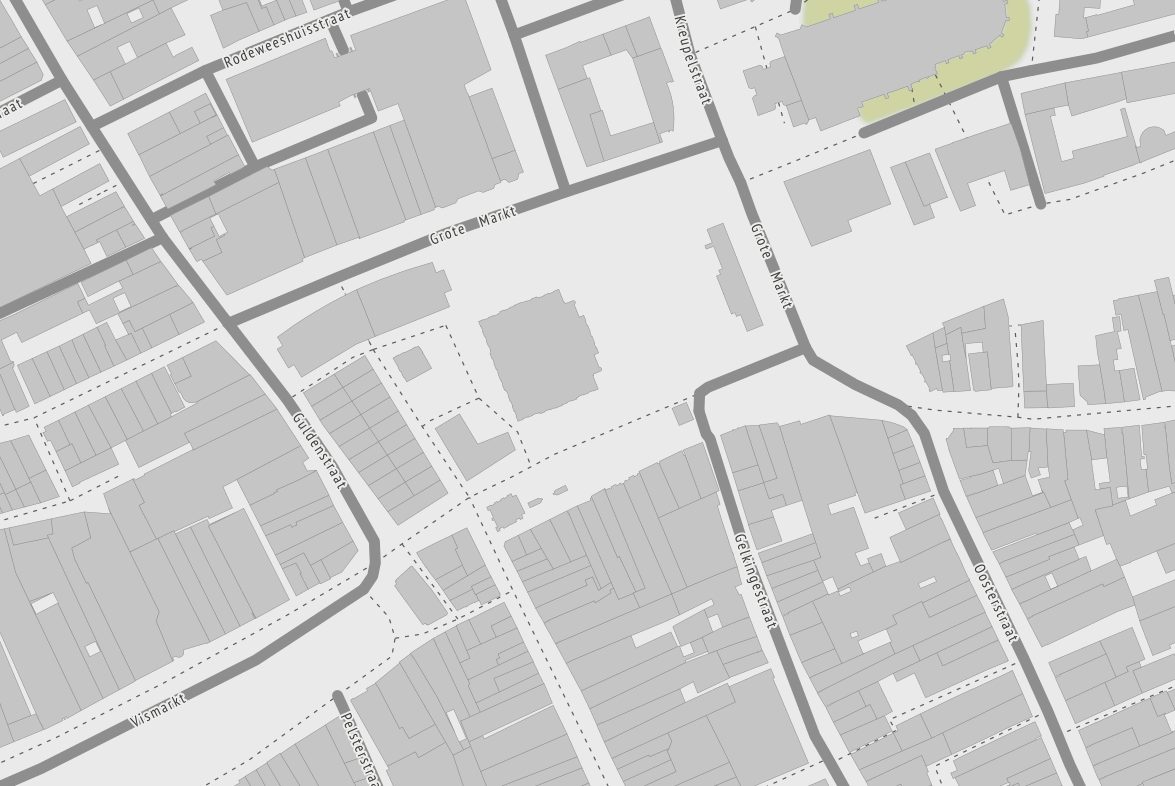
\includegraphics[width=0.8\linewidth]{../experiments/GroteMarktMaps/maps/groteMarkt.png}
\caption{Grote Markt.}
\end{subfigure}%
\begin{subfigure}{.5\textwidth}
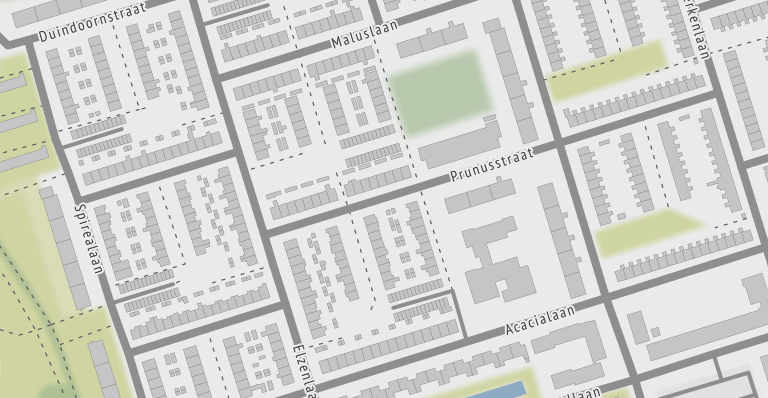
\includegraphics[width=0.8\linewidth]{../experiments/GroteMarktMaps/maps/Selwerd.png}
\caption{Selwerd.}
\end{subfigure}
\begin{subfigure}{.5\textwidth}
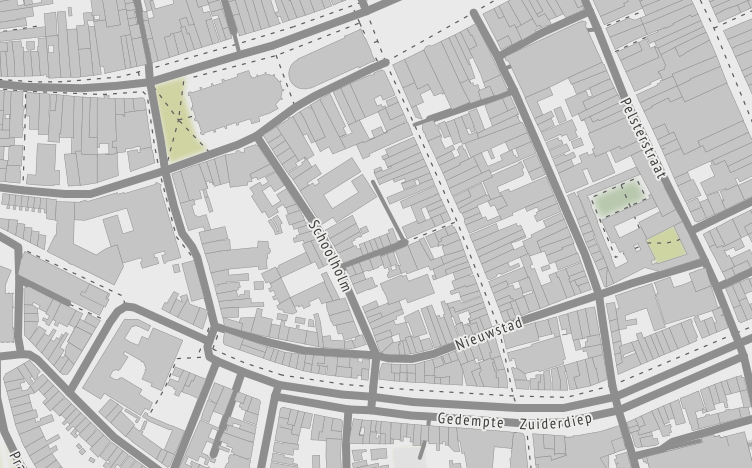
\includegraphics[width=0.8\linewidth]{../experiments/GroteMarktMaps/maps/zuidCentrum.png}
\caption{South-center}
\end{subfigure}%
\begin{subfigure}{.5\textwidth}
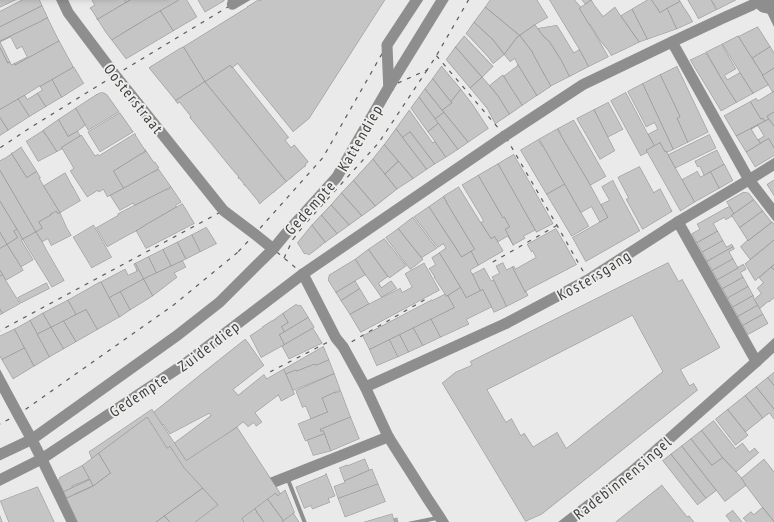
\includegraphics[width=0.8\linewidth]{../experiments/GroteMarktMaps/maps/kattediep.png}
\caption{Kattediep}
\end{subfigure}
\begin{subfigure}{.5\textwidth}
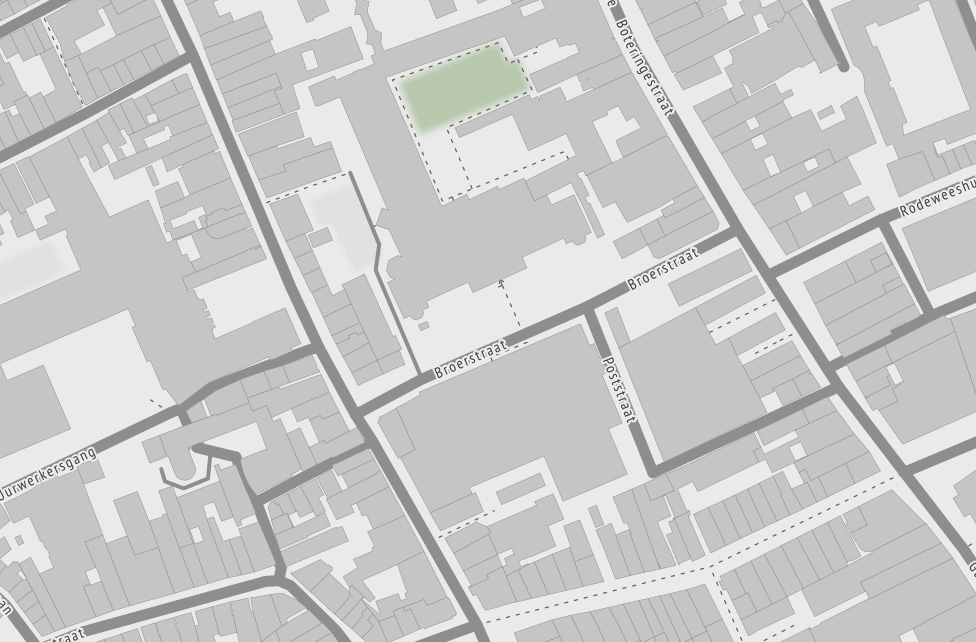
\includegraphics[width=0.8\linewidth]{../experiments/GroteMarktMaps/maps/academy.png}
\caption{Street with the academy building}
\end{subfigure}%
\begin{subfigure}{.5\textwidth}

\includegraphics[width=0.8\linewidth]{../experiments/GroteMarktMaps/maps/wall.png}
\caption{Not Groningen, just a wall}
\end{subfigure}
\caption{Maps.}
\label{maps}
\end{center}
\end{figure}


We look at the difference in the cpt tables for `seen\_1\_0', which represents the event that agent 1 (the thief), sees agent 0 (Table~\ref{mapstab}). If we did not need to condition on underlying geometry of the simulation, we would expect that this probability would be the same, regardless of map. However, we find something different - the probability of the thief seeing the potential victim, depends on the underlying map, and not just `a bit', the smallest probability is 0.19 for the GroteMarkt map, while the largest is 0.50 for the Wall Map. At this difference, robustness to rounding does not hold!

This means that we actually cannot speak of just one `probability' for the agent seeing the victim - we can only speak of the probability of the agent seeing the victim, as conditioned on the map. Implications of this is that we need to condition explicitly on maps for our networks to work, because it does meaningfully change the probabilities that we find, and there's no way to predict how the map that we're using affects the probabilities. This has implications for the real world, because it means that we can't depend on some generic ``probability of getting robbed'', we need to condition on spatial conditions/background world assumptions.

And these are not even very good maps - agents can either go somewhere, or not. Affordances in the real world are very different \footnote{parkour!}. So it's likely that the actual probabilities in the real world are even worse...



\begin{table}[]
\begin{tabular}{lllll}
map & accuracy & cpt of `seen\_1\_0' True \\
\hline
selwerd& 1 & 0.471\\
academy & 0.92 & 0.951\\
groteMarkt & 1 & 0.534\\
kattediep & 1 & 0.534\\
wall & 1 & 0.512\\
zuidCentrum &1 & 0.509\\
\end{tabular}
\caption{Difference in cpt depending only on difference in underlying map, no further difference in agent behaviour!}
\label{mapstab}
\end{table}


\subsection{Possible Legal Interpretations.}




